\documentclass[12pt]{report}
\usepackage{microtype}
\usepackage{cite}
\usepackage[english]{babel}
\usepackage{graphicx}

% -----------------------------------------------------------------------------
%                            custom macros
% -----------------------------------------------------------------------------

\newcommand{\HRule}{\rule{\linewidth}{0.5mm}}

% Remove the ugly ass chapter numbers
\makeatletter
\def\@makechapterhead#1{%
  \vspace*{-10\p@}%
  {\parindent \z@ \raggedright \normalfont
    %\ifnum \c@secnumdepth >\m@ne
    %    \huge\bfseries \@chapapp\space \thechapter
    %    \par\nobreak
    %    \vskip 20\p@
    %\fi
    \interlinepenalty\@M
    \Huge \bfseries #1\par\nobreak
    \vskip 10\p@
  }}
  \makeatother



% -----------------------------------------------------------------------------
%                           Title Page
% -----------------------------------------------------------------------------
\begin{document}
\begin{titlepage}
\begin{center}

% Upper part of the page. The '~' is needed because \\
% only works if a paragraph has started.
\textsc{\LARGE The University of Rochester}\\[1.0cm]

\textsc{\Large Area Paper}

for the Degree Master of Science\\[4cm]

% Title
\HRule \\[0.4cm]
{ \large \bfseries Binaural Audio as an Accessible User Interface }\\[0.4cm]

\HRule \\[0.5cm]

% Author and supervisor
\begin{minipage}{0.4\textwidth}
\begin{flushleft} \large
\emph{Author:}\\
Androwis \textsc{Abumoussa}
\end{flushleft}
\end{minipage}
\begin{minipage}{0.4\textwidth}
\begin{flushright} \large
\emph{Supervisor:} \\
Dr.~Jeffrey \textsc{Bigham}
\end{flushright}
\end{minipage}

\vfill

% Bottom of the page
{\large \today}

\end{center}
\end{titlepage}


% -----------------------------------------------------------------------------
%                            Table of Contents
% -----------------------------------------------------------------------------
\renewcommand{\thepage }{\roman{page}}
\tableofcontents

\newpage
\thispagestyle{empty}
\quad

% -----------------------------------------------------------------------------
%                           Acknowledgements
% -----------------------------------------------------------------------------
\newpage
\chapter{Acknowledgements}

% -----------------------------------------------------------------------------
%                           Abstract
% -----------------------------------------------------------------------------
\newpage
\chapter{Abstract}

% -----------------------------------------------------------------------------
%                           Introduction
% -----------------------------------------------------------------------------
\newpage
\renewcommand{\thepage }{\arabic{page}}
\setcounter{page}{1}
\chapter{Introduction}

Our society is driven by information.  Fields of research explore how to communicate constantly
changing information to interested parties at the appropriate time.  With the influx of mobile
devices that provide an always on channel, research has explored the effect these distruptions have
on a multitasking computing environment.  The goal of much of this research has been to study how
relevant and correct information can be efficiently delivered to a user in a manner that does not
distract from their current tasks\cite{McCrickard2003509}.

Armed with devices that are contstantly connected, our society has access to all sorts of information,
everything from weather forecasts and traffic conditions, to neighboring attractions,
restaurant schedules, store specials, even to the location and discoveries of our friends.

The essence of any event or update to user data is condensened into a notification.  Current
research has explored how notification systems attempt to deliver current, important information
to computer screens.  Many works have also explored the costs, benefits,
and optimal displays of these notifications from psychological prespectives that overlap
with our ability to handle interruptions and distractions~\cite{McCrickard2003509, cutrell2001notification}.

Given the stochastic nature of notifications, probabilistic reliability can be used to create
intelligent messaging sytems that gain a user's trust, rather than lose it~\cite{leetiernan2001effective}.
Emperical evidence show that users will ignore all notifications that are not highly valid when
performing demanding visual tasks~\cite{maltz2000cue}.

The question of a users trust in a system is therefore important when designing notification
interfaces, with the goal being mitigating all negative first impressions.  Empirical evidence shows that
users carry a historical bias when dealing with actionable notification \cite{leetiernan2001effective}.

The study of information design and options that are suitable for three often conflicting design objectives
of notifications - interruption to primary tasks, reactions to specific notificaitons, and comprehension
of information over time - are necessary.

\section{ Motivation }
Imagine driving to work on a typical morning. Eric Horvitz dream of an intelligent interface has been
realized, so your navigation system is checking current road conditions relative to
the location of the GPS inside of the car. Your smartphone has resumed polling your work
email address, your calendar has been updated by a colleague, and your family is
messaging you reminding you of a prior engagement.


 system that knew exactly how much or how little to say.  The system is able to
provide just the right amount of context for each task you're performing.

\section{ Binaural Audio}

Human auditory localization has been studied extensively~\cite{yost1987directional, blauert1997spatial}.
Humans are especially adept at localizing sounds in three dimensions.
Consider a sound source to the left of a listener.  Sounds from the
source arrive at the left ear first, and a short time after reach
the right ear.  The amplitude of the left ear sound will be attenuated
due to head shadowing.

The predominant audiotory cues for determining whether a sound is
coming from the left or right directions are the  interaural intensity
differences and the interaural time differences. Humans are also adept at
identifying sound position that are in front of or behind them, along
with estimating the sound source's elevation.  This is possible because
the incident sound waves interact with the torso, head, external ear
(pinna) prior to arriving at the inner ear.


The directional dependent filtering to each of a subject's ears can be
expressed as a frequency response, called a head related transfer function (HRTF),
and thus a pair of HRTFs describe how sound from one location reaches the two ears.
HRTFs are usually measured using human subjects or dummy-head microphones which
consist of response pairs for the left an right ears corresponding to a large number
of source positions surrounding the head.

\begin{figure}[h!]
  \centering
    \reflectbox{
      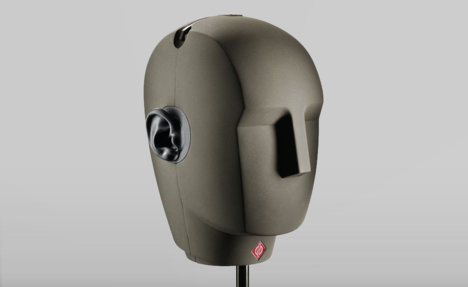
\includegraphics[width=.7\textwidth]{images/binaural_mic.png}
      }
  \caption{Binaural microphone with exact dimension and density as human head}
\end{figure}

There are two regions of interest when considering source locations of sound.  When the sound
is close to the head, the spherical curvature of the incident sound waves cause the HRTFs to change
qualitatively as a function of distance, but at moderate distances, the incident waves can be considered
planar. At extreme distances, humans are only capable to process auditory cues that only depend
on the sound sources volume.

Given that humans are capable of processing sound signals to place the audio source in space,
a binaural spatializer can then be implemented to simulate the auditory experience of one
or more sound sources arbitrarily located around a listener.  The general idea is reproduce
the acoustical signals at the two ears that would occur normally in a natural listening situation.

This process is accomplished by convolving each source signal with a pair of HRTFs corresponding to the
sound sources intended location.  The resulting signal is presented to the user through headphones.

\section{ Current Solutions}
\subsection {Transaural Audio}
Transaural audio is a method used to deliver signals to the ears of a listener using stereo loudspeakers.
The idea is to filter the binaural signal such that the subject can process the subsequent stereo
representation as a binaural signal.  This technique was first put into practice by Shroeder and Atal
~\cite{schroeder1963computer, schroeder1970digital}.
Song et al. demonstrated how computer vision techniques could be applied to the field of Transaural Audio. By tracking a subject's head, the computer can recalculate the HRTFs necessary for the sound,
as well as reposition the sound sources relative to the subject to provide an adaptive 3D audio system
~\cite{song2010personal}.

\section{ Research Domain}

\subsection { Audio Used for Analytics }
\subsection{ Audio Used for Interfaces }
\section{ Our Approach }

% -----------------------------------------------------------------------------
%                           Background
% -----------------------------------------------------------------------------
\newpage
\chapter{Background}
\section{ Audio's Role in Accessibility}
\section{ Current Audio Based Accessibility Solutions }

% -----------------------------------------------------------------------------
%                           Related Work
% -----------------------------------------------------------------------------
\newpage
\chapter{Related Work}
\section{ Interface Design}
\section{ Interfaces}
\section{ Engines}
\section{ Analytics }
\section{  }
\subsection{ Design Principles }
\subsection{ Design Patterns}
\subsection{ Design Methodologies }
\section{ Artificial Intelligence }


% -----------------------------------------------------------------------------
%                         Our Approach
% -----------------------------------------------------------------------------
\newpage
\chapter{Our Approach}


% -----------------------------------------------------------------------------
%                           Future Work
% -----------------------------------------------------------------------------
\newpage
\chapter{Future Work}
\section{ Analytics Domain }
\section{ Human Computer Interaction }



% -----------------------------------------------------------------------------
%                           Future Work
% -----------------------------------------------------------------------------
\newpage
\chapter{Conclusions}


% -----------------------------------------------------------------------------
%                           Future Work
% -----------------------------------------------------------------------------
\newpage
\bibliography{area}{}
\bibliographystyle{plain}



\end{document}             % End of document.